\documentclass[11pt]{report}
\usepackage{amsfonts}
\usepackage{fancyhdr}
\usepackage{comment}
\usepackage[a4paper, top=2.5cm, bottom=2.5cm, left=2.2cm, right=2.2cm]%{geometry}
\usepackage{times}
\usepackage{amsmath}
\usepackage{changepage}
\usepackage{amssymb}
\usepackage{graphicx}
\usepackage{titlesec}
\usepackage{lipsum}
\usepackage{dsfont}
\usepackage{listings}
\usepackage{tikz}
\usepackage{booktabs}
\graphicspath{{figures/}}
\titleformat{\chapter}[display]{\normalfont\bfseries}{}{0pt}{\Large}
\begin{document}
\title{Coursework 1}
\author{Shijun Luo \\22183515}
\date{\today}
\maketitle

\begin{figure}[h]
    \centering
    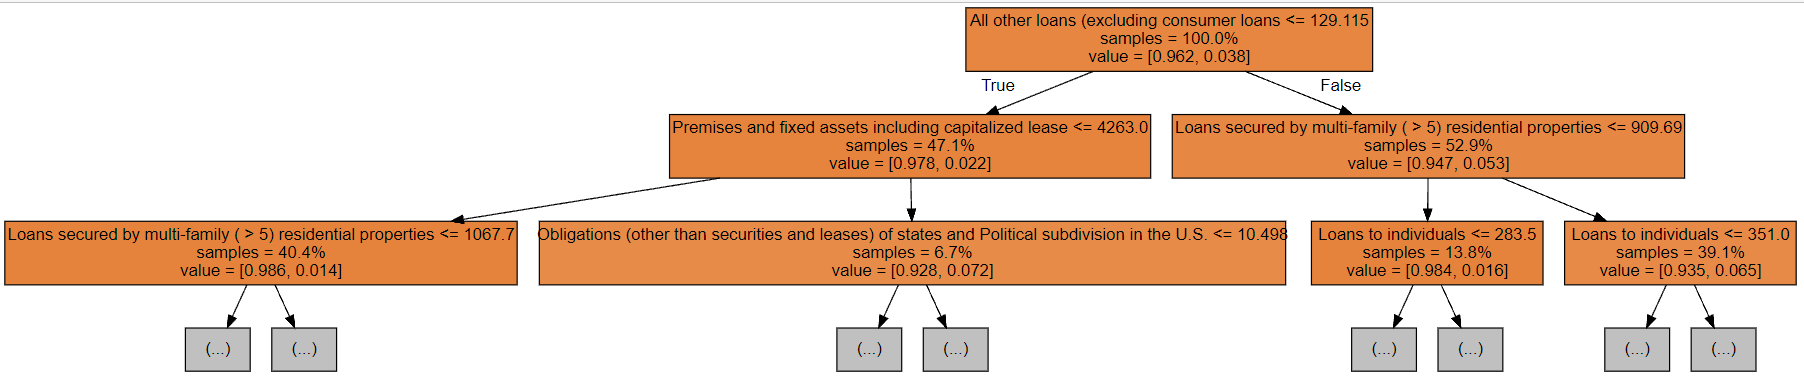
\includegraphics[width = \linewidth]{tree_1.png}
    \caption{Some examples of Classification Tree}\label{fig:tree_1}
\end{figure}

\begin{table}[h]
    \caption[table]{Report of Logistic Regression}
    \vspace{0.5em}\centering
    \begin{tabular}{ccccc}
        \toprule[1.5pt]
        &    precision    &recall  &f1-score   &support\\
        \midrule[1pt]                                   
        0       &0.97      &0.99      &0.98      &2243\\
        1       &0.41      &0.25      &0.31      &92\\
          & & & &                                   \\
 accuracy      &           &          &0.96      &2335\\
macro avg      & 0.69      &0.62      &0.64      &2335\\
weighted avg    &   0.95    &  0.96    &  0.95    &  2335\\
        \bottomrule[1.5pt]
    \end{tabular}
\end{table}

\end{document}